\documentclass[a4paper,10pt]{article}
\usepackage[utf8]{inputenc}
\usepackage{lipsum}
\usepackage{mathtools}
\usepackage{tikz}
\usepackage{pgfplots}
\usetikzlibrary{arrows,backgrounds,shapes,matrix,positioning,fit}
\usetikzlibrary{decorations.markings}
\usepackage{caption}
\usepackage{subcaption}
% For maths
\usepackage{amsmath}
\usepackage{amssymb}
% Set Margin
\usepackage[margin=1in]{geometry}
% For Figures
\usepackage{graphicx}
% For including source codes
\usepackage{listings}
\usepackage{color}
\definecolor{mygreen}{rgb}{0,0.6,0}
\definecolor{mygray}{rgb}{0.5,0.5,0.5}
\definecolor{mymauve}{rgb}{0.58,0,0.82}
\lstset{ %
  backgroundcolor=\color{white},   % choose the background color; you must add \usepackage{color} or \usepackage{xcolor}
  basicstyle=\footnotesize,        % the size of the fonts that are used for the code
  breakatwhitespace=false,         % sets if automatic breaks should only happen at whitespace
  breaklines=true,                 % sets automatic line breaking
  captionpos=b,                    % sets the caption-position to bottom
  commentstyle=\color{mygreen},    % comment style
  deletekeywords={...},            % if you want to delete keywords from the given language
  escapeinside={\%*}{*)},          % if you want to add LaTeX within your code
  extendedchars=true,              % lets you use non-ASCII characters; for 8-bits encodings only, does not work with UTF-8
  frame=single,                    % adds a frame around the code
  keepspaces=true,                 % keeps spaces in text, useful for keeping indentation of code (possibly needs columns=flexible)
  keywordstyle=\color{blue},       % keyword style
  language=Octave,                 % the language of the code
  morekeywords={*,...},            % if you want to add more keywords to the set
  numbers=left,                    % where to put the line-numbers; possible values are (none, left, right)
  numbersep=5pt,                   % how far the line-numbers are from the code
  numberstyle=\tiny\color{mygray}, % the style that is used for the line-numbers
  rulecolor=\color{black},         % if not set, the frame-color may be changed on line-breaks within not-black text (e.g. comments (green here))
  showspaces=false,                % show spaces everywhere adding particular underscores; it overrides 'showstringspaces'
  showstringspaces=false,          % underline spaces within strings only
  showtabs=false,                  % show tabs within strings adding particular underscores
  stepnumber=2,                    % the step between two line-numbers. If it's 1, each line will be numbered
  stringstyle=\color{mymauve},     % string literal style
  tabsize=2,                       % sets default tabsize to 2 spaces
  title=\lstname                   % show the filename of files included with \lstinputlisting; also try caption instead of title
}
\usepackage{caption}
\usepackage{url}
% for appendix
\usepackage[toc,page]{appendix}
\begin{document}

\pgfplotsset{compat=1.3}

%\tableofcontents

%\chapter{GNU Radio}

\section{GNU Radio}
GNU Radio\cite{bib:gnuradio} is a free \& open-source software development toolkit
that provides signal processing blocks to implement software radios.
It can be used with readily-available low-cost external RF hardware
to create software-defined radios, or without hardware in a simulation-like environment.
It is widely used in hobbyist, academic and commercial environments 
to support both wireless communications research and real-world radio systems.

A software radio is a radio system which performs the required signal processing 
in software instead of using dedicated integrated circuits in hardware.
The benefit is that since software can be easily replaced in the radio system,
the same hardware can be used to create many kinds of radios for many different transmission standards;
thus, one software radio can used for a variety of applications.

GNU Radio performs all the signal processing.
You can use it to write applications to receive data out of digital streams 
or to push data into digital streams, which is then transmitted using hardware.
GNU Radio has filters, channel codes, synchronization elements, equalizers,
demodulators, vocoders, decoders, and many other elements 
(in the GNU Radio jargon, we call these elements blocks) which are typically found in radio systems.
More importantly, it includes a method of connecting these blocks 
and then manages how data is passed from one block to another.
Extending GNU Radio is also quite easy; if you find a specific block that is missing, you can quickly create and add it.

Since GNU Radio is software, it can only handle digital data.
Usually, complex baseband samples are the input data type for receivers and the output data type for transmitters.
Analog hardware is then used to shift the signal to the desired center frequency.
That requirement aside, any data type can be passed from one block to another 
- be it bits, bytes, vectors, bursts or more complex data types.

GNU Radio applications are primarily written using the Python programming language, 
while the supplied, performance-critical signal processing path is implemented in C++
using processor floating point extensions, where available.
GNU Radio Companion(GRC) is a Simulink-like graphical tool to design signal processing flow-graphs.

GNU Radio supports several radio front-ends, either natively or through additional out-of-tree modules.
We will be using Ettus Research USRP platform and RTL-SDR TV tuners.

\subsection{First flow-graph}
Flow graphs are graphs (as in graph theory) through which data flows.
Many GNU Radio applications contain nothing other than a flow-graph.
The nodes of such a graph are called blocks, and the data flows along the edges.
The blocks are connected at ports. Data flows into or out of a block through these ports.

Any actual signal processing is done in the blocks.
Ideally, every block does exactly one job - this way GNU Radio stays modular and flexible.
Blocks are usually written in C++ (might also be Python); writing new blocks is not very difficult.

In order to illuminate this diffuse topic a little, let's start with an example.
Our aim is to generate a sinusoid and play it on audio output.
Open GNU Radio companion by executing gnuradio-companion on a terminal. 
Construct a flow-graph as shown in Figure \ref{fig:audio-play1}.

\begin{figure}[b]
\centering
 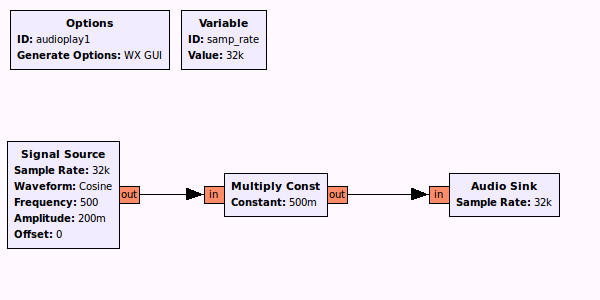
\includegraphics[scale=0.40]{figures/audio-play1.png}
 \caption{Playing 500Hz sinusoid on audio output.
 Take signal source and audio sink block from the list of blocks.
 Set the data type of signal source to float.
 Set the frequency to 500Hz and sampling rate to 32k.
 Set the sampling rate in the audio sink block to 32k.
 Connect these blocks and execute the flow-graph.\label{fig:audio-play1}}
\end{figure}
 
The first block has no input port. Such a block, with only output ports, is called a source. 
In an analog fashion, the final block, with no outputs, is called a sink.

So what's happening here?
The signal source produces samples of 500Hz cosine sampled at 32kHz per second.
The first 64 samples (which corresponds to a complete cycle of cosine in this case)
is plotted in Figure \ref{fig:signal-source-out}.
These samples are consumed by the multiply constant block,
which multiplies each of the input with 0.5.
Finally, the samples are passed to the audio output block which plays the incoming samples using computers audio card.
\begin{figure}
 \centering
 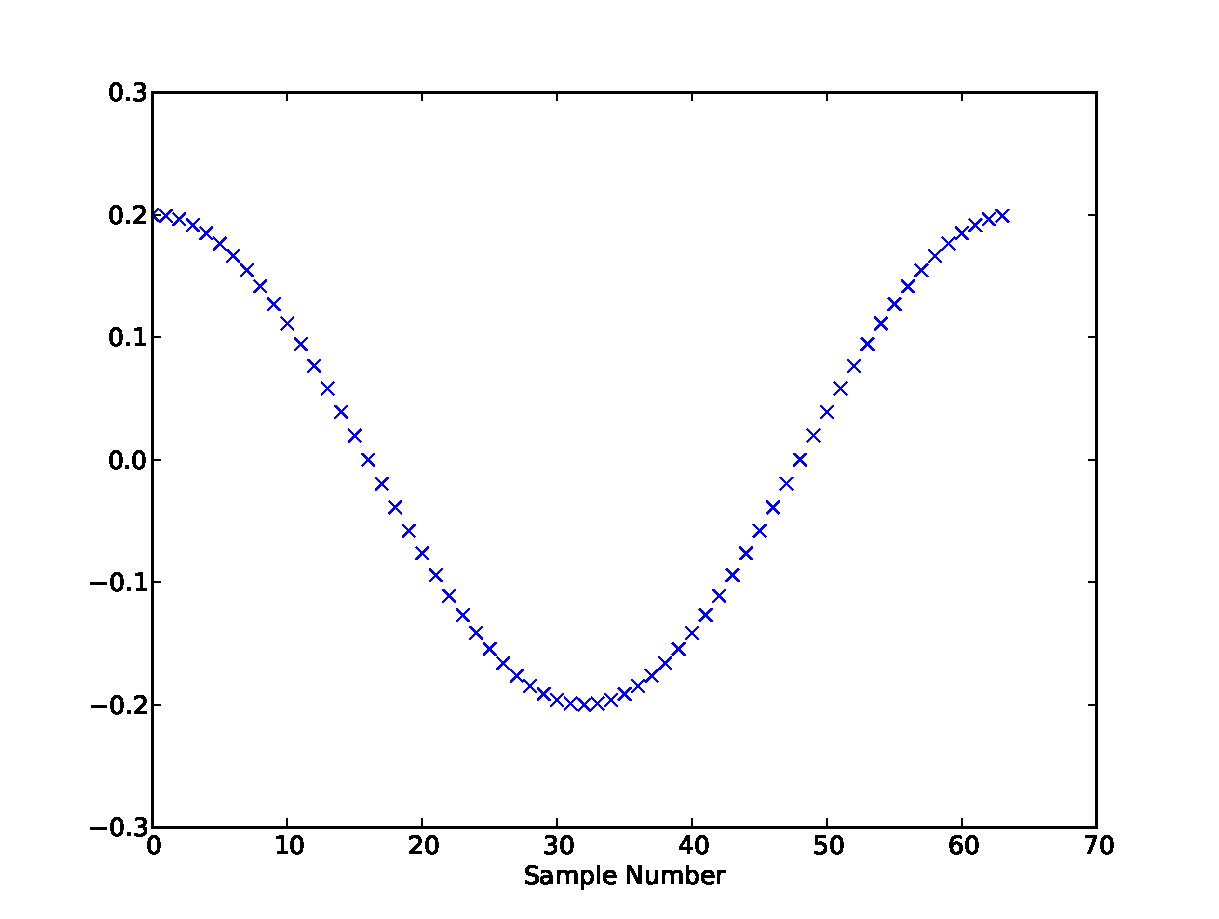
\includegraphics[scale=0.4]{figures/signal-source-out}
 \caption{The first 64 samples of output from the signal source. \label{fig:signal-source-out}}
\end{figure}

In general, we call whatever a block outputs/consumes, an item. 
In Figure \ref{fig:audio-play1}, one item was a float value representing one sample produced by the signal source. 
However, an item can be anything that can be represented digitally. 
The most common types of samples are real samples (as before), complex samples (the most common type in software defined radio), integer types, and vectors of these scalar types.

In Figure \ref{fig:audio-play1}, apart from playing the samples on audio card, everything else is done in software.
Since the audio card can only take specific sampling rates(32kHz, 44.1kHz, etc)
the rate at which the samples are processed through this flow-graph will be equal to the sampling rate of the audio card.

As mentioned before GNU Radio applications are written in python programming language. When we run any flow-graph
in GNU Radio companion, it is a python program that runs behind the scene. The python program corresponding to 
the flow-graph in Figure \ref{fig:audio-play1} is given in Listing \ref{lst:audio-play1}.
This program is auto-generated when we run the flow-graph in Figure \ref{fig:audio-play1} in grc.

Let us consider another example of computing the FFT of a signal source.
The flow-graph is given in Figure \ref{fig:compute-fft}.
In this example, the second block (stream to vector) produces one item(which is a vector of 1024 complex number) for every 1024 input items.
So, the rate at which it produces items is 1024 times smaller then the rate at which it consumes items 
(the fact that it actually produces bytes at the same rate it consumes them is irrelevant here).
Such a block is called a decimator, well, because it decimates the item rate. 
A block which outputs more items than it receives is called an interpolator. 
If it produces and consumes at the same rate, it's a sync block.
\begin{figure}
 \centering
 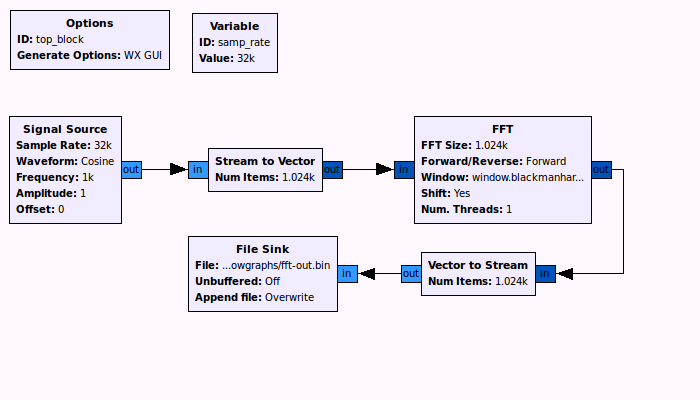
\includegraphics[scale=0.4]{figures/fft.png}
 \caption{Computing FFT \label{fig:compute-fft}}
\end{figure}

Let us ask the question what is the base sampling rate in Figure \ref{fig:compute-fft}?
Or how many complex numbers produced by the signal source, will be processed through this flow-graph in a second?
Well, we can't really answer this question.
In this flow-graph all that we are do, is to generate some numbers, do some math on the generated numbers, and save the output to a file.
As long as there is no hardware clock present which fixes the rate, 
sampling rate is meaningless--only relative rates (i.e. input to output rates are important. 
The computer may handle the samples as fast as it wants.
Note that this can cause the computer to lock up by allocating 100\% of CPU cycles to your signal processing.

In order to avoid the computer getting busy doing all the math, it is recommended to use a throttle block
when we run GNU Radio without any other hardware. The throttle block is tied to computer's hardware clock,
and it throttles the number of items passing through it.

Also when we have hardware involving different sampling rates, we might have to use some up-sampling/down-sampling
so that we meet the sampling rate requirement of all the hardwares.
\subsection{Complex data type in GNU Radio}
Most of the signal processing in GNU Radio is done on complex numbers.
In GNU Radio a complex number occupies 8 bytes in memory.
It actually consists of two 4-byte floats representing the real and imaginary components respectively.

\section{IQ Modulation\cite{bib:madhov}}
In RF communication we transmit our information in a small passband around a high frequency carrier.
All the information carried in a real-valued passband signal is contained in a corresponding complex-valued baseband signal. 
This baseband signal is called the complex baseband representation, or complex envelope, of the passband signal.
Any passband signal $s_{\text{p}}(t)$ can be written as
\begin{equation}
 s_{\text{p}}(t) = \sqrt{2}s_{\text{i}}(t)\operatorname{cos}(2\pi f_ct) - \sqrt{2}s_{\text{q}}(t)\operatorname{sin}(2\pi f_ct)
\end{equation}
where,
\begin{equation}
 s(t) = s_{\text{i}}(t) + \text{j}s_{\text{q}}(t)
\end{equation}
is called the complex envelope of $s_{\text{p}}(t)$. In GNU Radio we work with this complex envelope.
There are many hardwares available which can be interfaced with GNU Radio to transmit the output from a flow-graph
around any carrier that we may choose. Figure \ref{fig:complex-passband-spectrums} compares the spectrum of 
complex envelope and passband signals. Figure \ref{fig:upconversion} shows the process of IQ modulation.
Figure \ref{fig:downconversion} shows the process of IQ demodulation.

  \begin{figure}
    \centering
    \begin{subfigure}[t]{0.4\textwidth}
      \begin{tikzpicture}[scale=0.8,transform shape]
        \begin{axis}[
                     title=$\Re(S(f))$,
                     xmax=7,
                     xmin=-7,
                     ymax=1.5,
                     ymin=-1.1,
                     %axis lines = middle,
                     axis x line = middle,
                     axis y line = middle,
                     ytick=\empty,
                     xtick = {7},
                     xticklabels = {$f$},
                     %x tick label style={font=\tiny},
                     x post scale = 3.0
                    ]
          \addplot[color=blue,very thick] coordinates {(1,0) (-1,1.414) (-1,0)};
        \end{axis}
      \end{tikzpicture}
  \end{subfigure}
  \begin{subfigure}[t]{0.4\textwidth}
      \begin{tikzpicture}[scale=0.8,transform shape]
        \begin{axis}[
                     title=$\Im(S(f))$,
                     xmax=7,
                     xmin=-7,
                     ymax=1.5,
                     ymin=-1.1,
                     %axis lines = middle,
                     axis x line = middle,
                     axis y line = middle,
                     ytick=\empty,
                     xtick = {7},
                     xticklabels = {$f$},
                     %x tick label style={font=\tiny},
                     x post scale = 3.0
                    ]
          \addplot[color=blue,very thick] coordinates {(1,0) (1,1.414) (-1,1.414) (-1,0)};
        \end{axis}
      \end{tikzpicture}
  \end{subfigure}
  \begin{subfigure}[b]{0.4\textwidth}
      \begin{tikzpicture}[scale=0.8,transform shape]
        \begin{axis}[
                     title=$\Re(S_{\text{p}}(f))$,
                     xmax=7,
                     xmin=-7,
                     ymax=1.5,
                     ymin=-1.1,
                     %axis lines = middle,
                     axis x line = middle,
                     axis y line = middle,
                     ytick=\empty,
                     xtick = {-5,5,7},
                     xticklabels = {$-f_c$,$f_c$,$f$},
                     %x tick label style={font=\tiny},
                     x post scale = 3.0
                    ]
          \addplot[color=blue,very thick] coordinates {(-6,0) (-4,1) (-4,0)};
          \addplot[color=blue,very thick] coordinates {(6,0) (4,1) (4,0)};
        \end{axis}
      \end{tikzpicture}
  \end{subfigure}
  \begin{subfigure}[b]{0.4\textwidth}
      \begin{tikzpicture}[scale=0.8,transform shape]
        \begin{axis}[
                     title=$\Im(S_{\text{p}}(f))$,
                     xmax=7,
                     xmin=-7,
                     ymax=1.5,
                     ymin=-1.1,
                     %axis lines = middle,
                     axis x line = middle,
                     axis y line = middle,
                     ytick=\empty,
                     xtick = {-5,5,7},
                     xticklabels = {$-f_c$,$f_c$,$f$},
                     %x tick label style={font=\tiny},
                     x post scale = 3.0
                    ]
          \addplot[color=blue,very thick] coordinates {(-6,0) (-6,-1) (-4,-1) (-4,0)};
          \addplot[color=blue,very thick] coordinates {(6,0) (6,1) (4,1) (4,0)};
        \end{axis}
      \end{tikzpicture}
  \end{subfigure}
  \caption{Spectrum of complex envelope and passband signals \label{fig:complex-passband-spectrums}}
  \end{figure}
  
    \begin{figure}
    \centering
      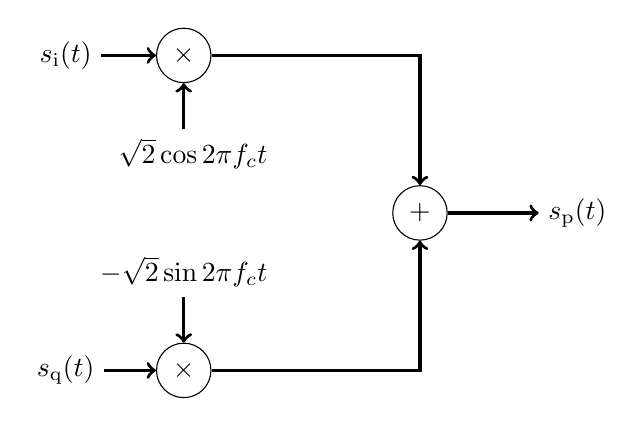
\begin{tikzpicture}[scale=1.0,transform shape]
      \node at (-0.5,2) (sc) {$s_{\text{i}}(t)$};
      \node at (-0.5,-2) (ss) {$s_{\text{q}}(t)$};
      \node[circle, draw, minimum size = 5mm] at (1,2) (prodc) {$\times$};
      \node[circle, draw, minimum size = 5mm] at (1,-2) (prods) {$\times$};
      \node[circle, draw, minimum size = 5mm] at (4,0) (adder) {$+$};
      \node at (1,0.75) (cos) {$\ \ \sqrt{2}\cos 2\pi f_ct$};
      \node at (1,-0.75) (sin) {$-\sqrt{2}\sin 2\pi f_ct$};
      \node at (6,0) (sp) {$s_{\text{p}}(t)$};
      \draw[->,very thick] (sc) -- (prodc);
      \draw[->,very thick] (ss) -- (prods);
      \draw[->,very thick] (prodc) -| (adder);
      \draw[->,very thick] (prods) -| (adder);
      \draw[->,very thick] (cos) -- (prodc);
      \draw[->,very thick] (sin) -- (prods);
      \draw[->,very thick] (adder) -- (sp);
      \end{tikzpicture}
   \caption{Up-conversion: Getting passband signal from complex envelope
   \label{fig:upconversion}}
  \end{figure}
  
    \begin{figure}
    \centering
      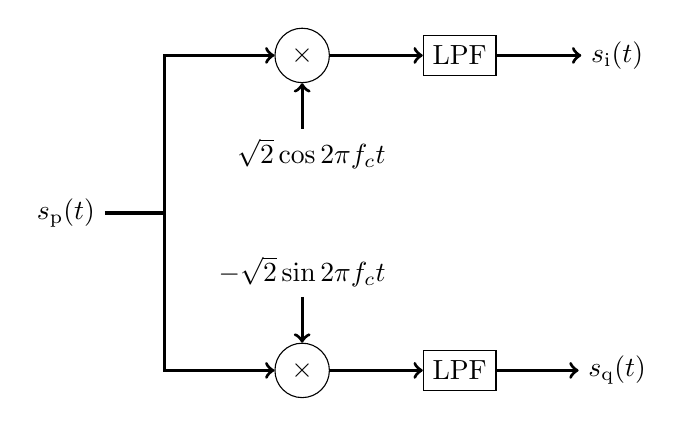
\begin{tikzpicture}[scale=1.0,transform shape]
      \node at (5,2) (sc) {$s_{\text{i}}(t)$};
      \node at (5,-2) (ss) {$s_{\text{q}}(t)$};
      \node[circle, draw, minimum size = 5mm] at (1,2) (prodc) {$\times$};
      \node[circle, draw, minimum size = 5mm] at (1,-2) (prods) {$\times$};
      \node[rectangle, draw, minimum size = 5mm] at (3,2) (LPc) {LPF};
      \node[rectangle, draw, minimum size = 5mm] at (3,-2) (LPs) {LPF};
      \node at (1,0.75) (cos) {$\ \ \sqrt{2}\cos 2\pi f_ct$};
      \node at (1,-0.75) (sin) {$-\sqrt{2}\sin 2\pi f_ct$};
      \node at (-2,0) (sp) {$s_{\text{p}}(t)$};
      \draw[->,very thick] (prodc) -- (LPc);
      \draw[->,very thick] (prods) -- (LPs);
      \draw[->,very thick] (LPc) -- (sc);
      \draw[->,very thick] (LPs) -- (ss);
      \draw[->,very thick] (cos) -- (prodc);
      \draw[->,very thick] (sin) -- (prods);
      \draw[->,very thick] (-0.75,0) |- (prodc);
      \draw[->,very thick] (-0.75,0) |- (prods);
      \draw[very thick] (sp) -- (-0.75,0);
      \end{tikzpicture}
      \caption{Down-conversion: Getting the complex envelope from passband
      \label{fig:downconversion}}
  \end{figure}

\section{IQ Modulator Board}
We have developed an IQ modulator board at Wadhwani Electronics Labs.
This IQ modulator board features Linear Technology's LTC5598 modulator LTC6946-1 synthesizer and PIC18F4550 micro-controller.
With the combination of these chips the IQ modulator can transmit in the range 373MHz - 1600MHz.
The block diagram of this board is given in Figure \ref{fig:board-block-diagram}.
\begin{figure}
\centering
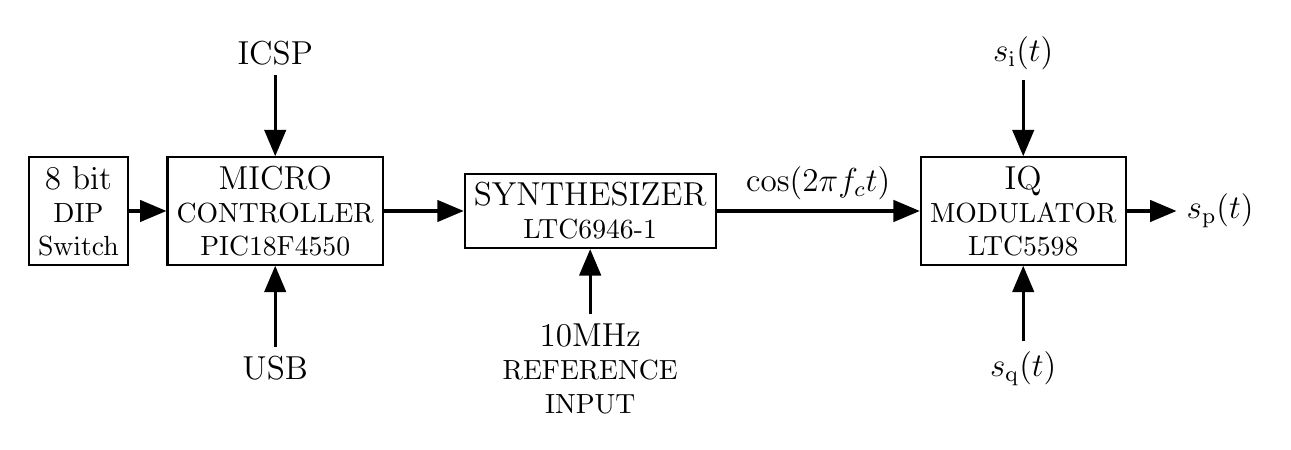
\begin{tikzpicture}[auto, thick, node distance=2cm, >=triangle 45, every text node part/.style={align=center}]
\draw
  node at (-2.5, 0)[draw, thick, rectangle](switch){\large 8 bit \\ DIP \\ Switch}
  node at (0, 2)(jtag) {\large ICSP}
  node at (0,0)[draw, thick, rectangle](uc){\large MICRO \\ CONTROLLER \\ \normalsize PIC18F4550 }
  node at (0, -2)(usb) {\large USB}
  node at (4,0)[draw, thick, rectangle](pll){\large SYNTHESIZER \\ \normalsize LTC6946-1}
  node at (4,-2)(refin){\large 10MHz \\ REFERENCE \\ INPUT}
  node at (9.5,2) (sit){\large $s_{\text{i}}(t)$}
  node at (9.5,-2) (sqt){\large $s_{\text{q}}(t)$}
  node at (12,0)(rf){\large $s_{\text{p}}(t)$}
  node at (9.5,0)[draw, thick, rectangle](mod){\large IQ \\ MODULATOR \\ \normalsize LTC5598};
  \draw[->,very thick] (jtag) -- (uc);
  \draw[->,very thick] (usb) -- (uc);
  \draw[->,very thick] (uc) -- (pll);
  \draw[->,very thick] (pll) -- node[above] {\large $\cos(2\pi f_ct)$} (mod);
  \draw[->,very thick] (refin) -- (pll);
  \draw[->,very thick] (sit) -- (mod);
  \draw[->,very thick] (sqt) -- (mod);
  \draw[->,very thick] (mod) -- (rf);
  \draw[->,very thick] (switch) -- (uc);
\end{tikzpicture}
\caption{Block diagram of IQ modulator board \label{fig:board-block-diagram}}
\end{figure}

LTC 5598\cite{bib:modchip}
is a high linearity direct quadrature modulator, which works in the range from 5MHz to 1600MHz. 
It allows direct modulation of an RF signal using differential I and Q signals.
The internal block digram of LTC5598 is given in Figure \ref{fig:mod-block}.
The baseband input $s_{\text{i}}(t)$ is fed through the differential pair BBPI(pin 21) and BBMI(pin 22).
The baseband input $s_{\text{q}}(t)$ is fed through the differential pair BBPQ(pin 10) and BBMQ(pin 9).
The I/Q baseband inputs consist of voltage-to-current converters that in turn drive double-balanced mixers.
The outputs of these mixers are summed and applied to a buffer,
which converts the differential mixer signals to a $50\Omega$ single-ended buffered RF output.
\begin{figure}
\centering
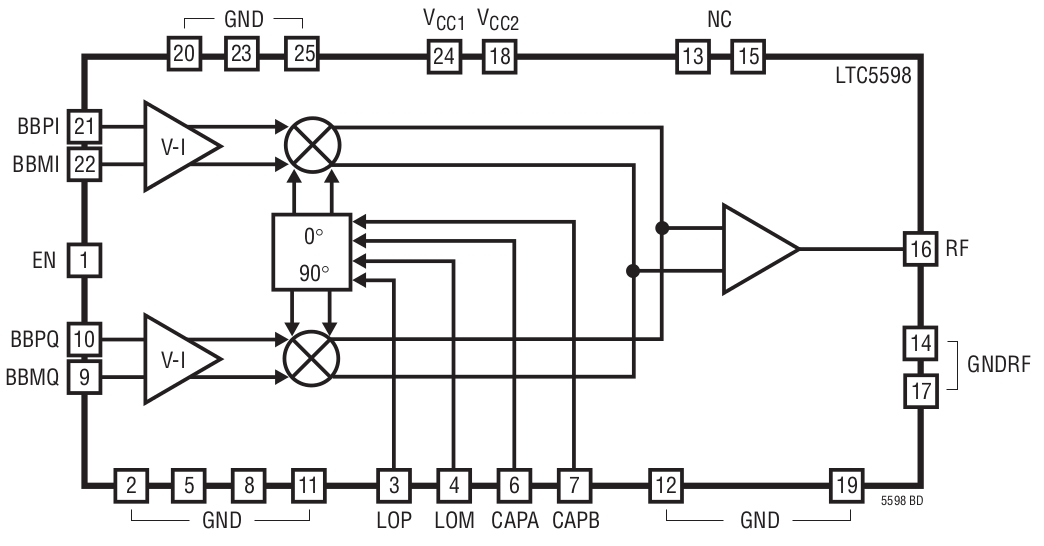
\includegraphics[scale=0.4]{figures/ltc5598-block-diagram.jpg}
\caption{Internal block digram of LTC5598 chip. \label{fig:mod-block}}
\end{figure}
The four balanced I and Q baseband input ports are intended for DC coupling from a source with a common-mode voltage level of about 0.5V.
We will be generating our baseband inputs $s_{\text{i}}(t)$ and $s_{\text{q}}(t)$ from a two channel arbitrary function generator.
Since these signals are single ended, we will be feeding BBPI with $s_{\text{i}}(t)$ and BBPQ wit $s_{\text{q}}(t)$.
A DC offset(0.5 typical) should be added with $s_{\text{i}}(t)$ and $s_{\text{q}}(t)$ at the AFG to meet common mode voltage requirement.
Their differential pair BBMI and BBMQ are tied to a DC voltage(0.5V fixed/0-0.6V adjustable depending on jumper setting) on the board.
The LO path consists of an LO buffer with single-ended or differential inputs, and precision
quadrature generators that produce the LO drive for the mixers.
In our design, the carrier at $f_c$(LO) generated from LTC6946-1 is fed through the LOP and LOM differential inputs.
The passband output $s_{\text{p}}(t)$ can be fed to an antenna from the RF(pin 16) output.

LTC6946-1\cite{bib:pllchip} is a high performance, low noise phase-locked loop (PLL) with a fully integrated VCO,
including a reference divider, phase-frequency detector (PFD) with phase-lock indicator,
ultralow noise charge pump, integer feedback divider, and VCO output divider.
It's frequency range is from 373MHz to 3740MHz.
The RF$^-$ and the RF$^+$ outputs from the PLL are respectively connected to the LOM and LOP input of the modulator.
The internal block diagram of LTC6946-1 is given in Figure \ref{fig:pll-block}.
\begin{figure}
\centering
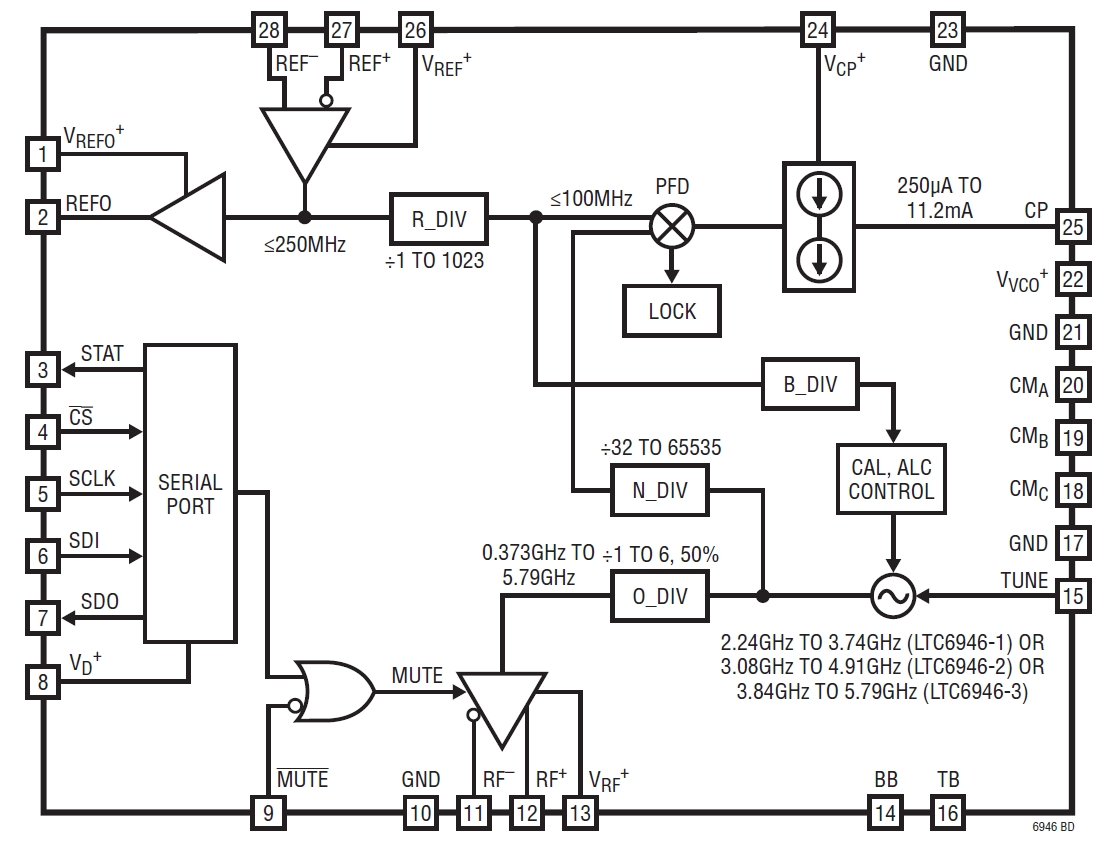
\includegraphics[scale=0.4]{figures/pll-block-diagram.jpg}
\caption{Internal block digram of LTC6946 chip. \label{fig:pll-block}}
\end{figure}

In our design the reference input of the PLL is fed from a 10MHz crystal oscillator at the REF$^+$(pin 27) input.
There are 12 registers in the PLL. We name them h00 to h0B.
These registers can be written of read through the chip's SPI compatible serial port.
We use PIC18F4550 as the SPI controller.
The output frequency is controlled by values in the register.
A 10-bit divider, R\_DIV, is used to reduce the frequency seen at the PFD.
Its divide ratio $R$ may be set to any integer from 1 to 1023, inclusive.
The 16-bit N-divider provides the feedback from the VCO to the PFD.
Its divide ratio $N$ may be set to any integer from 32 to 65535, inclusive.
The 3-bit O-divider can reduce the frequency from the VCO
to extend the output frequency range. Its divide ratio $O$
may be set to any integer from 1 to 6, inclusive, outputting a 50\% duty cycle even with odd divide values.
The frequency at RF$^\pm$ is given by
\begin{equation}
 f_{\text{RF}} = \frac{f_{\text{REF}}*N}{O*R}
\end{equation}

The PIC18F4550 which is the SPI master, loads the registers in the PLL with default configuration at the system startup.
We have defined the following default configuration values among others.
\begin{align*}
 R &= 4 \\
 O &= 5
\end{align*}
With these settings, when the $N$ value changes by 1, the $f_{\text{RF}}$ changes by $f_{\text{STEP}}$, where
\begin{align}
 f_{\text{STEP}} &= \frac{f_{\text{REF}}}{O*R} \\
		  &= \frac{10}{4*5}\text{MHz} \nonumber \\
                 &= 500\text{kHz} \nonumber
\end{align}
The $N$ value can be changed using the 8 bit DIP switch.
The switch setting $S~ \in ~\lbrace 0, 1, \cdots, 255 \rbrace$ is read by the micro-controller.
The default program defines the base value $N_0$ of $N$ to be 0x0380(890).
The value of $N$ is given by
\begin{equation}
 N = N_0 + S
\end{equation}
Thus with the default settings we can generate $f_c$, where
\begin{align}
 f_c &= f_{\text{STEP}}*(890 + S)\text{kHz},~~S~ \in ~\lbrace 0, 1, \cdots, 255 \rbrace \nonumber \\
     &= (448 + 0.5S)\text{MHz},~~S~ \in ~\lbrace 0, 1, \cdots, 255 \rbrace
\end{align}

One can modify the default settings in the PLL by programming the micro-controller, and can tune to other frequencies.
The details of how to program the PLL is given in \cite{bib:pllchip}. We have provided ICSP interface and USB interface
for programming the micro-controller.

\section{RTL-SDR Dongles\cite{bib:rtlsdr}}
Realtek RTL2832U DVB-T tuner dongles are used for DAB/DAB+/FM demodulation.
Since the RTL2832U chip allows transferring the raw I/Q samples to the host, it can be used as a cheap SDR.
The RTL2832U outputs 8-bit I/Q-samples, and the highest theoretically possible sample-rate is 3.2 MS/s.
So theoretically it can capture a signals of upto 3.2MHz passband bandwidth.
We usually work at lower sampling rates, so that samples are not lost.
The frequency range of operation is determined by the tuner in the circuit.
The dongles in our lab have Rafael Micro tuner, whose frequency range of operation is 24 - 1766 MHz.

In short these dongles do what is shown in Figure \ref{fig:downconversion}
and gives the samples of $s_{\text{i}}(t)$ and $s_{\text{q}}(t)$ to the host computer.
A GNU Radio flow-graph in the host computer can read these samples and these samples can be processed using various DSP algorithms in GNU Radio,
to extract the embedded information.

\section{Universal Software Radio Peripheral(USRP)\cite{bib:usrp}}
USRP is a software radio platform, which usually have both transmit and receive capabilities.
USRP can be directly interfaced with a computer through USB of Gigabit Ethernet.
When used as a transmitter a USRP essentially do what is shown in Figure \ref{fig:upconversion},
in addition to generation of both of both the $s_{\text{i}}(t)$ and $s_{\text{q}}(t)$,
from their respective samples supplied by the host computer, through digital to analog conversion.
When used a receiver, a USRP essentially do what is shown in Figure \ref{fig:downconversion} and
gives the samples of $s_{\text{i}}(t)$ and $s_{\text{q}}(t)$ to the host computer.

In our lab we will be using USRP B100 series. B100 USRPs have USB 2.0 interface.
We can set the sample width to 8-bits or 16-bits.
With 8 bit sample width, each of I and Q sample takes 8 bits each, and thus a complex sample in total takes 16 bits.
With 16 bit sample width, each of I and Q sample takes 16 bits each, and thus a complex sample in total takes 32 bits.
The speed of of USB 2.0 interface is 480Mbps.
So we can get maximum sampling rate of 30MS/s at 8 bit sample width.
Thus we can capture/send messages of bandwidth upto 30MHz.
With 16 bit sample width we can get maximum sampling rate of 15MS/s,
limiting our maximum bandwidth to 15MHz.

The frequency range of operation of the USRP is determined by the RF daughter board attached.
In the labs we will be using WBX daughter boards which can operate in 50 MHz to 2.2 GHz range.

\newpage
\ifx\du\undefined
  \newlength{\du}
\fi
\setlength{\du}{15\unitlength}
\begin{figure}
 \begin{tikzpicture}
\pgftransformxscale{1.000000}
\pgftransformyscale{-1.000000}
\definecolor{dialinecolor}{rgb}{0.000000, 0.000000, 0.000000}
\pgfsetstrokecolor{dialinecolor}
\definecolor{dialinecolor}{rgb}{1.000000, 1.000000, 1.000000}
\pgfsetfillcolor{dialinecolor}
\definecolor{dialinecolor}{rgb}{1.000000, 1.000000, 1.000000}
\pgfsetfillcolor{dialinecolor}
\fill (8.783333\du,2.137500\du)--(8.783333\du,4.837500\du)--(12.783333\du,4.837500\du)--(12.783333\du,2.137500\du)--cycle;
\pgfsetlinewidth{0.100000\du}
\pgfsetdash{}{0pt}
\pgfsetdash{}{0pt}
\pgfsetmiterjoin
\definecolor{dialinecolor}{rgb}{0.000000, 0.000000, 0.000000}
\pgfsetstrokecolor{dialinecolor}
\draw (8.783333\du,2.137500\du)--(8.783333\du,4.837500\du)--(12.783333\du,4.837500\du)--(12.783333\du,2.137500\du)--cycle;
% setfont left to latex
\definecolor{dialinecolor}{rgb}{0.000000, 0.000000, 0.000000}
\pgfsetstrokecolor{dialinecolor}
\node at (10.783333\du,3.282500\du){Phase};
% setfont left to latex
\definecolor{dialinecolor}{rgb}{0.000000, 0.000000, 0.000000}
\pgfsetstrokecolor{dialinecolor}
\node at (10.783333\du,4.082500\du){Detector};
\definecolor{dialinecolor}{rgb}{1.000000, 1.000000, 1.000000}
\pgfsetfillcolor{dialinecolor}
\fill (-6.536667\du,2.175000\du)--(-6.536667\du,4.875000\du)--(-2.196667\du,4.875000\du)--(-2.196667\du,2.175000\du)--cycle;
\pgfsetlinewidth{0.100000\du}
\pgfsetdash{}{0pt}
\pgfsetdash{}{0pt}
\pgfsetmiterjoin
\definecolor{dialinecolor}{rgb}{0.000000, 0.000000, 0.000000}
\pgfsetstrokecolor{dialinecolor}
\draw (-6.536667\du,2.175000\du)--(-6.536667\du,4.875000\du)--(-2.196667\du,4.875000\du)--(-2.196667\du,2.175000\du)--cycle;
% setfont left to latex
\definecolor{dialinecolor}{rgb}{0.000000, 0.000000, 0.000000}
\pgfsetstrokecolor{dialinecolor}
\node at (-4.366667\du,3.320000\du){TCXO};
% setfont left to latex
\definecolor{dialinecolor}{rgb}{0.000000, 0.000000, 0.000000}
\pgfsetstrokecolor{dialinecolor}
\node at (-4.366667\du,4.120000\du){10 MHz};
\definecolor{dialinecolor}{rgb}{1.000000, 1.000000, 1.000000}
\pgfsetfillcolor{dialinecolor}
\fill (14.560193\du,1.079983\du)--(14.560193\du,5.879983\du)--(16.792693\du,5.879983\du)--(16.792693\du,1.079983\du)--cycle;
\pgfsetlinewidth{0.100000\du}
\pgfsetdash{}{0pt}
\pgfsetdash{}{0pt}
\pgfsetmiterjoin
\definecolor{dialinecolor}{rgb}{0.000000, 0.000000, 0.000000}
\pgfsetstrokecolor{dialinecolor}
\draw (14.560193\du,1.079983\du)--(14.560193\du,5.879983\du)--(16.792693\du,5.879983\du)--(16.792693\du,1.079983\du)--cycle;
% setfont left to latex
\definecolor{dialinecolor}{rgb}{0.000000, 0.000000, 0.000000}
\pgfsetstrokecolor{dialinecolor}
\node at (15.676443\du,3.674983\du){};
\definecolor{dialinecolor}{rgb}{1.000000, 1.000000, 1.000000}
\pgfsetfillcolor{dialinecolor}
\pgfpathellipse{\pgfpoint{15.674820\du}{2.229313\du}}{\pgfpoint{0.753592\du}{0\du}}{\pgfpoint{0\du}{0.931867\du}}
\pgfusepath{fill}
\pgfsetlinewidth{0.100000\du}
\pgfsetdash{}{0pt}
\pgfsetdash{}{0pt}
\pgfsetmiterjoin
\definecolor{dialinecolor}{rgb}{0.000000, 0.000000, 0.000000}
\pgfsetstrokecolor{dialinecolor}
\pgfpathellipse{\pgfpoint{15.674820\du}{2.229313\du}}{\pgfpoint{0.753592\du}{0\du}}{\pgfpoint{0\du}{0.931867\du}}
\pgfusepath{stroke}
% setfont left to latex
\definecolor{dialinecolor}{rgb}{0.000000, 0.000000, 0.000000}
\pgfsetstrokecolor{dialinecolor}
\node at (15.674820\du,2.424313\du){};
\definecolor{dialinecolor}{rgb}{1.000000, 1.000000, 1.000000}
\pgfsetfillcolor{dialinecolor}
\pgfpathellipse{\pgfpoint{15.689504\du}{4.758100\du}}{\pgfpoint{0.753592\du}{0\du}}{\pgfpoint{0\du}{0.931867\du}}
\pgfusepath{fill}
\pgfsetlinewidth{0.100000\du}
\pgfsetdash{}{0pt}
\pgfsetdash{}{0pt}
\pgfsetmiterjoin
\definecolor{dialinecolor}{rgb}{0.000000, 0.000000, 0.000000}
\pgfsetstrokecolor{dialinecolor}
\pgfpathellipse{\pgfpoint{15.689504\du}{4.758100\du}}{\pgfpoint{0.753592\du}{0\du}}{\pgfpoint{0\du}{0.931867\du}}
\pgfusepath{stroke}
% setfont left to latex
\definecolor{dialinecolor}{rgb}{0.000000, 0.000000, 0.000000}
\pgfsetstrokecolor{dialinecolor}
\node at (15.689504\du,4.953100\du){};
\pgfsetlinewidth{0.100000\du}
\pgfsetdash{}{0pt}
\pgfsetdash{}{0pt}
\pgfsetbuttcap
{
\definecolor{dialinecolor}{rgb}{0.000000, 0.000000, 0.000000}
\pgfsetfillcolor{dialinecolor}
% was here!!!
\pgfsetarrowsend{stealth}
\definecolor{dialinecolor}{rgb}{0.000000, 0.000000, 0.000000}
\pgfsetstrokecolor{dialinecolor}
\draw (15.674820\du,1.297446\du)--(15.674820\du,3.161180\du);
}
\pgfsetlinewidth{0.100000\du}
\pgfsetdash{}{0pt}
\pgfsetdash{}{0pt}
\pgfsetbuttcap
{
\definecolor{dialinecolor}{rgb}{0.000000, 0.000000, 0.000000}
\pgfsetfillcolor{dialinecolor}
% was here!!!
\pgfsetarrowsend{stealth}
\definecolor{dialinecolor}{rgb}{0.000000, 0.000000, 0.000000}
\pgfsetstrokecolor{dialinecolor}
\draw (15.689504\du,3.826233\du)--(15.689504\du,5.689967\du);
}
\pgfsetlinewidth{0.100000\du}
\pgfsetdash{}{0pt}
\pgfsetdash{}{0pt}
\pgfsetbuttcap
{
\definecolor{dialinecolor}{rgb}{0.000000, 0.000000, 0.000000}
\pgfsetfillcolor{dialinecolor}
% was here!!!
\pgfsetarrowsend{stealth}
\definecolor{dialinecolor}{rgb}{0.000000, 0.000000, 0.000000}
\pgfsetstrokecolor{dialinecolor}
\draw (12.783333\du,3.487500\du)--(14.560193\du,3.479983\du);
}
\pgfsetlinewidth{0.100000\du}
\pgfsetdash{}{0pt}
\pgfsetdash{}{0pt}
\pgfsetbuttcap
{
\definecolor{dialinecolor}{rgb}{0.000000, 0.000000, 0.000000}
\pgfsetfillcolor{dialinecolor}
% was here!!!
\definecolor{dialinecolor}{rgb}{0.000000, 0.000000, 0.000000}
\pgfsetstrokecolor{dialinecolor}
\draw (15.674820\du,3.161180\du)--(15.680484\du,3.777179\du);
}
% setfont left to latex
\definecolor{dialinecolor}{rgb}{0.000000, 0.000000, 0.000000}
\pgfsetstrokecolor{dialinecolor}
\node[anchor=west] at (17.266667\du,3.450000\du){};
\definecolor{dialinecolor}{rgb}{1.000000, 1.000000, 1.000000}
\pgfsetfillcolor{dialinecolor}
\fill (20.565000\du,2.131250\du)--(20.565000\du,4.831250\du)--(23.247500\du,4.831250\du)--(23.247500\du,2.131250\du)--cycle;
\pgfsetlinewidth{0.100000\du}
\pgfsetdash{}{0pt}
\pgfsetdash{}{0pt}
\pgfsetmiterjoin
\definecolor{dialinecolor}{rgb}{0.000000, 0.000000, 0.000000}
\pgfsetstrokecolor{dialinecolor}
\draw (20.565000\du,2.131250\du)--(20.565000\du,4.831250\du)--(23.247500\du,4.831250\du)--(23.247500\du,2.131250\du)--cycle;
% setfont left to latex
\definecolor{dialinecolor}{rgb}{0.000000, 0.000000, 0.000000}
\pgfsetstrokecolor{dialinecolor}
\node at (21.906250\du,3.276250\du){Loop};
% setfont left to latex
\definecolor{dialinecolor}{rgb}{0.000000, 0.000000, 0.000000}
\pgfsetstrokecolor{dialinecolor}
\node at (21.906250\du,4.076250\du){Filter};
\definecolor{dialinecolor}{rgb}{1.000000, 1.000000, 1.000000}
\pgfsetfillcolor{dialinecolor}
\fill (1.803750\du,2.158333\du)--(1.803750\du,4.858333\du)--(5.196250\du,4.858333\du)--(5.196250\du,2.158333\du)--cycle;
\pgfsetlinewidth{0.100000\du}
\pgfsetdash{}{0pt}
\pgfsetdash{}{0pt}
\pgfsetmiterjoin
\definecolor{dialinecolor}{rgb}{0.000000, 0.000000, 0.000000}
\pgfsetstrokecolor{dialinecolor}
\draw (1.803750\du,2.158333\du)--(1.803750\du,4.858333\du)--(5.196250\du,4.858333\du)--(5.196250\du,2.158333\du)--cycle;
% setfont left to latex
\definecolor{dialinecolor}{rgb}{0.000000, 0.000000, 0.000000}
\pgfsetstrokecolor{dialinecolor}
\node at (3.500000\du,3.303333\du){R};
% setfont left to latex
\definecolor{dialinecolor}{rgb}{0.000000, 0.000000, 0.000000}
\pgfsetstrokecolor{dialinecolor}
\node at (3.500000\du,4.103333\du){Divider};
\definecolor{dialinecolor}{rgb}{1.000000, 1.000000, 1.000000}
\pgfsetfillcolor{dialinecolor}
\fill (7.753750\du,6.008333\du)--(7.753750\du,8.708333\du)--(11.146250\du,8.708333\du)--(11.146250\du,6.008333\du)--cycle;
\pgfsetlinewidth{0.100000\du}
\pgfsetdash{}{0pt}
\pgfsetdash{}{0pt}
\pgfsetmiterjoin
\definecolor{dialinecolor}{rgb}{0.000000, 0.000000, 0.000000}
\pgfsetstrokecolor{dialinecolor}
\draw (7.753750\du,6.008333\du)--(7.753750\du,8.708333\du)--(11.146250\du,8.708333\du)--(11.146250\du,6.008333\du)--cycle;
% setfont left to latex
\definecolor{dialinecolor}{rgb}{0.000000, 0.000000, 0.000000}
\pgfsetstrokecolor{dialinecolor}
\node at (9.450000\du,7.153333\du){N};
% setfont left to latex
\definecolor{dialinecolor}{rgb}{0.000000, 0.000000, 0.000000}
\pgfsetstrokecolor{dialinecolor}
\node at (9.450000\du,7.953333\du){Divider};
\pgfsetlinewidth{0.100000\du}
\pgfsetdash{}{0pt}
\pgfsetdash{}{0pt}
\pgfsetbuttcap
{
\definecolor{dialinecolor}{rgb}{0.000000, 0.000000, 0.000000}
\pgfsetfillcolor{dialinecolor}
% was here!!!
\pgfsetarrowsend{stealth}
\definecolor{dialinecolor}{rgb}{0.000000, 0.000000, 0.000000}
\pgfsetstrokecolor{dialinecolor}
\draw (9.450000\du,6.008333\du)--(10.783333\du,4.837500\du);
}
\definecolor{dialinecolor}{rgb}{1.000000, 1.000000, 1.000000}
\pgfsetfillcolor{dialinecolor}
\fill (12.339988\du,9.262500\du)--(12.339988\du,11.162500\du)--(14.829988\du,11.162500\du)--(14.829988\du,9.262500\du)--cycle;
\pgfsetlinewidth{0.100000\du}
\pgfsetdash{}{0pt}
\pgfsetdash{}{0pt}
\pgfsetmiterjoin
\definecolor{dialinecolor}{rgb}{0.000000, 0.000000, 0.000000}
\pgfsetstrokecolor{dialinecolor}
\draw (12.339988\du,9.262500\du)--(12.339988\du,11.162500\du)--(14.829988\du,11.162500\du)--(14.829988\du,9.262500\du)--cycle;
% setfont left to latex
\definecolor{dialinecolor}{rgb}{0.000000, 0.000000, 0.000000}
\pgfsetstrokecolor{dialinecolor}
\node at (13.584988\du,10.407500\du){VCO};
\pgfsetlinewidth{0.100000\du}
\pgfsetdash{}{0pt}
\pgfsetdash{}{0pt}
\pgfsetbuttcap
{
\definecolor{dialinecolor}{rgb}{0.000000, 0.000000, 0.000000}
\pgfsetfillcolor{dialinecolor}
% was here!!!
\pgfsetarrowsend{stealth}
\definecolor{dialinecolor}{rgb}{0.000000, 0.000000, 0.000000}
\pgfsetstrokecolor{dialinecolor}
\draw (16.792693\du,3.479983\du)--(22.698333\du,3.481250\du);
}
\pgfsetlinewidth{0.100000\du}
\pgfsetdash{}{0pt}
\pgfsetdash{}{0pt}
\pgfsetmiterjoin
\pgfsetbuttcap
{
\definecolor{dialinecolor}{rgb}{0.000000, 0.000000, 0.000000}
\pgfsetfillcolor{dialinecolor}
% was here!!!
{\pgfsetcornersarced{\pgfpoint{0.000000\du}{0.000000\du}}\definecolor{dialinecolor}{rgb}{0.000000, 0.000000, 0.000000}
\pgfsetstrokecolor{dialinecolor}
\draw (1.000000\du,4.000000\du)--(1.000000\du,12.000000\du);
}}
\pgfsetlinewidth{0.100000\du}
\pgfsetdash{}{0pt}
\pgfsetdash{}{0pt}
\pgfsetmiterjoin
\pgfsetbuttcap
{
\definecolor{dialinecolor}{rgb}{0.000000, 0.000000, 0.000000}
\pgfsetfillcolor{dialinecolor}
% was here!!!
{\pgfsetcornersarced{\pgfpoint{0.000000\du}{0.000000\du}}\definecolor{dialinecolor}{rgb}{0.000000, 0.000000, 0.000000}
\pgfsetstrokecolor{dialinecolor}
\draw (1.000000\du,12.000000\du)--(16.600000\du,12.000000\du);
}}
\pgfsetlinewidth{0.100000\du}
\pgfsetdash{}{0pt}
\pgfsetdash{}{0pt}
\pgfsetmiterjoin
\pgfsetbuttcap
{
\definecolor{dialinecolor}{rgb}{0.000000, 0.000000, 0.000000}
\pgfsetfillcolor{dialinecolor}
% was here!!!
{\pgfsetcornersarced{\pgfpoint{0.000000\du}{0.000000\du}}\definecolor{dialinecolor}{rgb}{0.000000, 0.000000, 0.000000}
\pgfsetstrokecolor{dialinecolor}
\draw (17.133333\du,12.000000\du)--(17.133333\du,0.600000\du);
}}
\pgfsetlinewidth{0.100000\du}
\pgfsetdash{}{0pt}
\pgfsetdash{}{0pt}
\pgfsetmiterjoin
\pgfsetbuttcap
{
\definecolor{dialinecolor}{rgb}{0.000000, 0.000000, 0.000000}
\pgfsetfillcolor{dialinecolor}
% was here!!!
{\pgfsetcornersarced{\pgfpoint{0.000000\du}{0.000000\du}}\definecolor{dialinecolor}{rgb}{0.000000, 0.000000, 0.000000}
\pgfsetstrokecolor{dialinecolor}
\draw (18.733333\du,0.600000\du)--(3.133333\du,0.600000\du);
}}
\pgfsetlinewidth{0.100000\du}
\pgfsetdash{}{0pt}
\pgfsetdash{}{0pt}
\pgfsetmiterjoin
\pgfsetbuttcap
{
\definecolor{dialinecolor}{rgb}{0.000000, 0.000000, 0.000000}
\pgfsetfillcolor{dialinecolor}
% was here!!!
{\pgfsetcornersarced{\pgfpoint{0.000000\du}{0.000000\du}}\definecolor{dialinecolor}{rgb}{0.000000, 0.000000, 0.000000}
\pgfsetstrokecolor{dialinecolor}
\draw (1.000000\du,0.600000\du)--(1.000000\du,4.000000\du);
}}
\pgfsetlinewidth{0.100000\du}
\pgfsetdash{}{0pt}
\pgfsetdash{}{0pt}
\pgfsetbuttcap
{
\definecolor{dialinecolor}{rgb}{0.000000, 0.000000, 0.000000}
\pgfsetfillcolor{dialinecolor}
% was here!!!
\definecolor{dialinecolor}{rgb}{0.000000, 0.000000, 0.000000}
\pgfsetstrokecolor{dialinecolor}
\draw (21.906250\du,4.831250\du)--(19.000000\du,10.200000\du);
}
\pgfsetlinewidth{0.100000\du}
\pgfsetdash{}{0pt}
\pgfsetdash{}{0pt}
\pgfsetbuttcap
{
\definecolor{dialinecolor}{rgb}{0.000000, 0.000000, 0.000000}
\pgfsetfillcolor{dialinecolor}
% was here!!!
\pgfsetarrowsend{stealth}
\definecolor{dialinecolor}{rgb}{0.000000, 0.000000, 0.000000}
\pgfsetstrokecolor{dialinecolor}
\draw (19.000000\du,10.200000\du)--(14.829988\du,10.212500\du);
}
\definecolor{dialinecolor}{rgb}{1.000000, 1.000000, 1.000000}
\pgfsetfillcolor{dialinecolor}
\fill (2.253750\du,8.866667\du)--(2.253750\du,11.566667\du)--(5.646250\du,11.566667\du)--(5.646250\du,8.866667\du)--cycle;
\pgfsetlinewidth{0.100000\du}
\pgfsetdash{}{0pt}
\pgfsetdash{}{0pt}
\pgfsetmiterjoin
\definecolor{dialinecolor}{rgb}{0.000000, 0.000000, 0.000000}
\pgfsetstrokecolor{dialinecolor}
\draw (2.253750\du,8.866667\du)--(2.253750\du,11.566667\du)--(5.646250\du,11.566667\du)--(5.646250\du,8.866667\du)--cycle;
% setfont left to latex
\definecolor{dialinecolor}{rgb}{0.000000, 0.000000, 0.000000}
\pgfsetstrokecolor{dialinecolor}
\node at (3.950000\du,10.011667\du){O};
% setfont left to latex
\definecolor{dialinecolor}{rgb}{0.000000, 0.000000, 0.000000}
\pgfsetstrokecolor{dialinecolor}
\node at (3.950000\du,10.811667\du){Divider};
\pgfsetlinewidth{0.100000\du}
\pgfsetdash{}{0pt}
\pgfsetdash{}{0pt}
\pgfsetbuttcap
{
\definecolor{dialinecolor}{rgb}{0.000000, 0.000000, 0.000000}
\pgfsetfillcolor{dialinecolor}
% was here!!!
\pgfsetarrowsend{stealth}
\definecolor{dialinecolor}{rgb}{0.000000, 0.000000, 0.000000}
\pgfsetstrokecolor{dialinecolor}
\draw (-2.196667\du,3.525000\du)--(1.803750\du,3.508333\du);
}
\pgfsetlinewidth{0.100000\du}
\pgfsetdash{}{0pt}
\pgfsetdash{}{0pt}
\pgfsetbuttcap
{
\definecolor{dialinecolor}{rgb}{0.000000, 0.000000, 0.000000}
\pgfsetfillcolor{dialinecolor}
% was here!!!
\pgfsetarrowsend{stealth}
\definecolor{dialinecolor}{rgb}{0.000000, 0.000000, 0.000000}
\pgfsetstrokecolor{dialinecolor}
\draw (12.289807\du,10.213180\du)--(5.646250\du,10.216667\du);
}
\pgfsetlinewidth{0.100000\du}
\pgfsetdash{}{0pt}
\pgfsetdash{}{0pt}
\pgfsetbuttcap
{
\definecolor{dialinecolor}{rgb}{0.000000, 0.000000, 0.000000}
\pgfsetfillcolor{dialinecolor}
% was here!!!
\pgfsetarrowsend{stealth}
\definecolor{dialinecolor}{rgb}{0.000000, 0.000000, 0.000000}
\pgfsetstrokecolor{dialinecolor}
\draw (9.525000\du,10.200000\du)--(9.525000\du,8.700000\du);
}
\pgfsetlinewidth{0.100000\du}
\pgfsetdash{}{0pt}
\pgfsetdash{}{0pt}
\pgfsetbuttcap
{
\definecolor{dialinecolor}{rgb}{0.000000, 0.000000, 0.000000}
\pgfsetfillcolor{dialinecolor}
% was here!!!
\pgfsetarrowsend{stealth}
\definecolor{dialinecolor}{rgb}{0.000000, 0.000000, 0.000000}
\pgfsetstrokecolor{dialinecolor}
\draw (5.196250\du,3.508333\du)--(8.783333\du,3.487500\du);
}
% setfont left to latex
\definecolor{dialinecolor}{rgb}{0.000000, 0.000000, 0.000000}
\pgfsetstrokecolor{dialinecolor}
\node[anchor=west] at (6.000000\du,3.200000\du){$f_{\text{PFD}}$};
\end{tikzpicture}
\end{figure}


\newpage
%%% References
\begin{thebibliography}{9}
 \bibitem{bib:gnuradio}
 \url{http://gnuradio.org}
 \bibitem{bib:modchip}
 \url{http://www.linear.com/product/LTC5598} 
 \bibitem{bib:pllchip}
 \url{http://www.linear.com/product/LTC6946} 
 
 \bibitem{bib:madhov} Upamanyu Madhov, ``Fundamentals of Digital Communication'', CUP 2008.
 \bibitem{bib:rtlsdr}
 \url{http://sdr.osmocom.org/trac/wiki/rtl-sdr}
 \bibitem{bib:usrp}
 \url{http://www.ettus.com/home}
 \end{thebibliography}

\newpage
\begin{appendices}
\lstinputlisting[language=Python, caption=The python program corresponding to the flow-graph in Figure \ref{fig:audio-play1}, label=lst:audio-play1]
{flowgraphs/audioplay1.py}
\end{appendices}

\end{document}


